%%========================================================================
%% LaTeX sjabloon voor stage/projectrapport of bachelorproef
%%  HoGent Bedrijf en Organisatie
%%========================================================================

%%========================================================================
%% Preamble
%%========================================================================

\documentclass[pdftex,a4paper,12pt,twoside]{report}

% XXX: Let op: dit sjabloon is gemaakt om dubbelzijdig af te drukken
% Voor enkelzijdig, verwijder ``twoside'' hierboven.

%%---------- Extra functionaliteit ---------------------------------------

\usepackage[utf8]{inputenc}  % Accenten gebruiken in tekst (vb. é ipv \'e)
\usepackage{amsfonts}        % AMS math packages: extra wiskundige
\usepackage{amsmath}         %   symbolen (o.a. getallen-
\usepackage{amssymb}         %   verzamelingen N, R, Z, Q, etc.)
%\usepackage[dutch]{babel}   % Taalinstellingen: woordsplitsingen,
                             %  commando's voor speciale karakters
                             %  ("dutch" voor NL)
\usepackage{eurosym}         % Euro-symbool €
\usepackage{geometry}
\usepackage{graphicx}        % Invoegen van tekeningen
\usepackage[hyphens]{url}
\usepackage[pdftex,bookmarks=true,hidelinks]{hyperref}
                             % PDF krijgt klikbare links & verwijzingen,
                             %  inhoudstafel
\usepackage{epigraph}
\usepackage{listings}        % Broncode mooi opmaken
\usepackage{multirow}        % Tekst over verschillende cellen in tabellen
\usepackage{rotating}        % Tabellen en figuren roteren
\usepackage{natbib}          % Betere bibliografiestijlen
\usepackage{fancyhdr}        % Pagina-opmaak met hoofd- en voettekst

\usepackage[T1]{fontenc}     % Ivm lettertypes
\usepackage{lmodern}
\usepackage{textcomp}
\usepackage{tikz}
\usepackage{pgfplots}

%%---------- Layout ------------------------------------------------------

% hoofdingen, enz.
\pagestyle{fancy}
% enkel hoofdstuktitel in hoofding, geen sectietitel (vermijd overlap)
\renewcommand{\sectionmark}[1]{}

% lijn, wordt gebruikt in titelpagina
\newcommand{\HRule}{\rule{\linewidth}{0.5mm}}

% Leeg blad
\newcommand{\emptypage}{
\newpage
\thispagestyle{empty}
\mbox{}
\newpage
}

% Gebruik een schreefloos lettertype ipv het "oubollig" uitziende
% Computer Modern
\renewcommand{\familydefault}{\sfdefault}

% Commando voor invoegen Java-broncodebestanden (dank aan Niels Corneille)
% Gebruik: \codefragment{source/MijnKlasse.java}{Uitleg bij de code}
\newcommand{\codefragment}[2]{ \lstset{%
  language=java,
  breaklines=true,
  float=th,
  caption={#2},
  basicstyle=\scriptsize,
  frame=single,
  extendedchars=\true
}
\lstinputlisting{#1}}

%%---------- Documenteigenschappen ---------------------------------------
%% Vul dit aan met je eigen info:

% Je eigen naam
\newcommand{\student}{Jan {Van Braeckel}}

% De naam van je lector, begeleider, promotor
\newcommand{\promotor}{Joeri {Van Herreweghe}}

% De naam van je co-promotor
\newcommand{\copromotor}{Peter Leemans}

% Indien je bachelorproef in opdracht van een bedrijf of organisatie
% geschreven is, geef je hier de naam.
\newcommand{\instelling}{AllThingsTalk}

% De titel van het rapport/bachelorproef
\newcommand{\titel}{Bluetooth Low Energy wearables in een Internet of Things cloud-infrastructuur met behulp van een smartphone als gateway}
\newcommand{\titleEN}{Bluetooth Low Energy wearables in an Internet of Things cloud infrastructure using a smartphone as gateway}

% Datum van indienen
\newcommand{\datum}{27 mei 2015}

% Faculteit
\newcommand{\faculteit}{Faculteit `Bedrijf en Organisatie'}
\newcommand{\faculty}{Faculty `Bedrijf en Organisatie'}

% Soort rapport
\newcommand{\rapporttype}{Scriptie voorgedragen tot het bekomen van de graad\\Bachelor in de toegepaste informatica}
\newcommand{\reporttype}{Thesis submitted in fulfilment of the requirements for the degree of\\Bachelor in applied computer sciences}

% Academiejaar
\newcommand{\academiejaar}{2015-2016}

% Examenperiode
%  - 1e semester = 1e examenperiode
%  - 2e semester = 2e examenperiode
%  - tweede zit = 3e examenperiode
\newcommand{\examenperiode}{Tweede examenperiode}
\newcommand{\examperiod}{Second exam period}

%%========================================================================
%% Inhoud document
%%========================================================================

\begin{document}

%%---------- Front matter ------------------------------------------------
%% Het voorblad - Hier moet je in principe niets wijzigen.

\begin{titlepage}
  \newgeometry{top=2cm,bottom=1.5cm,left=1.5cm,right=1.5cm}
  \begin{center}

    \begingroup
    \rmfamily
    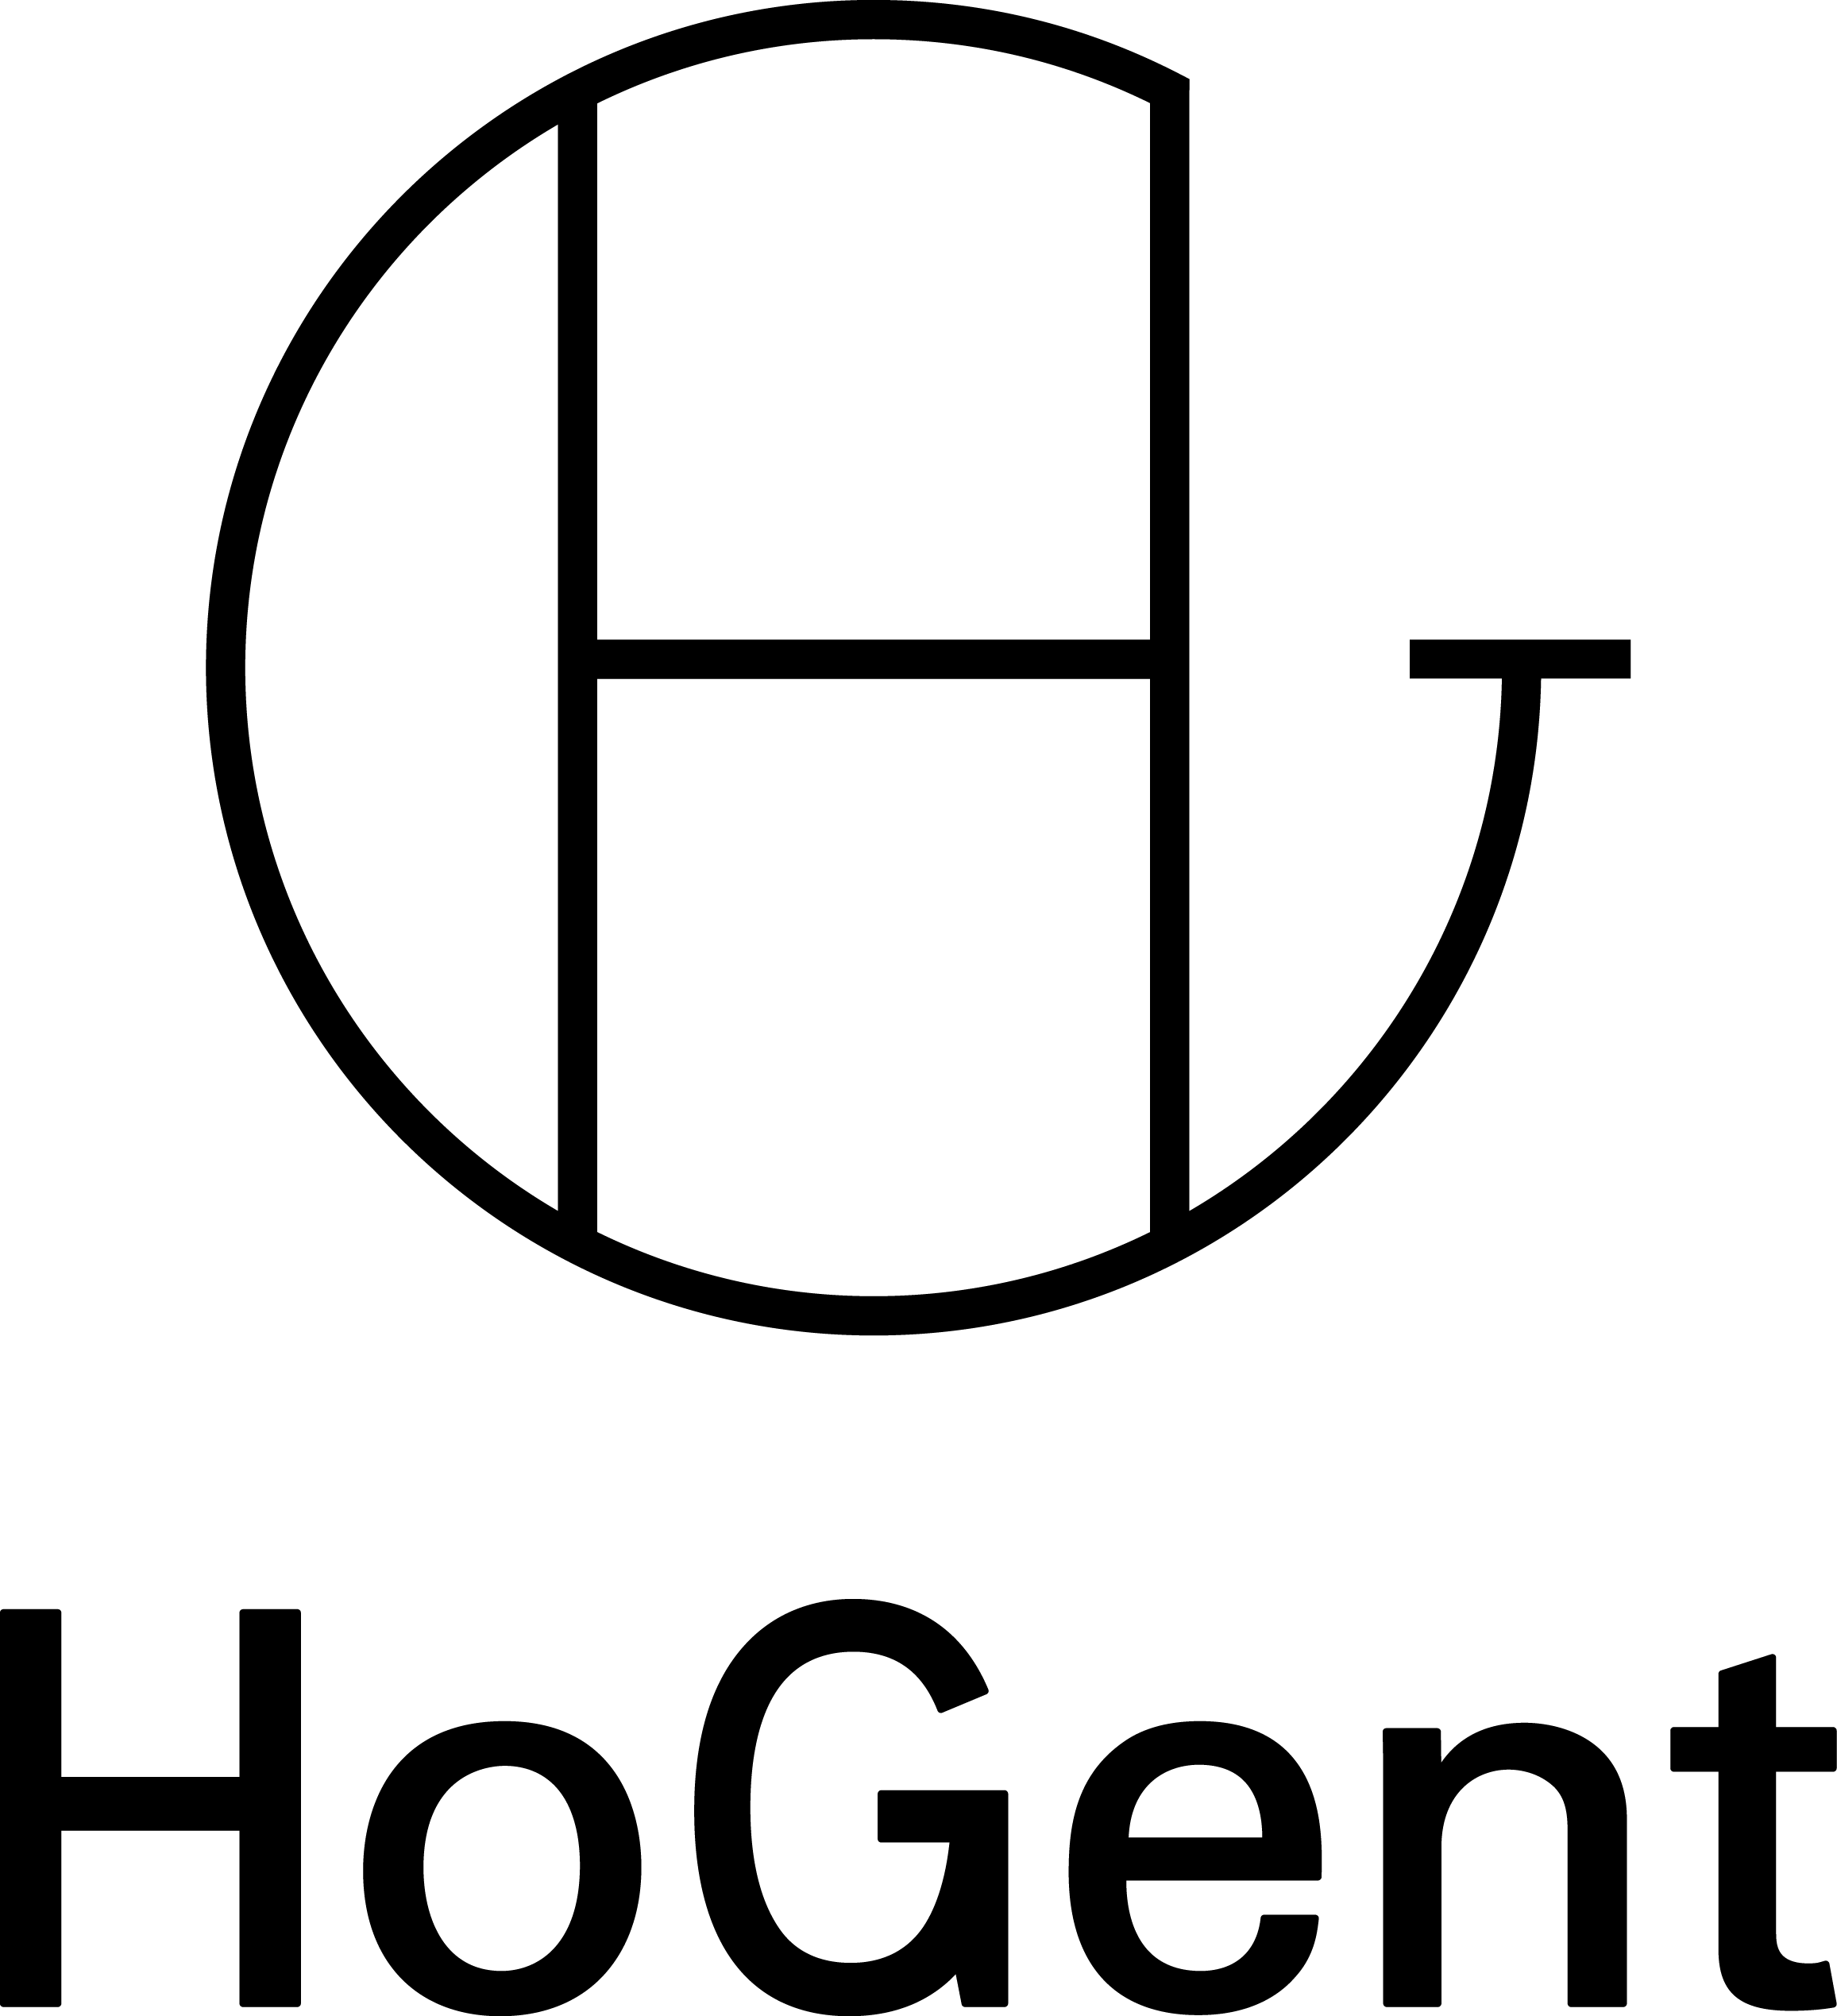
\includegraphics[width=2.5cm]{img/HG-beeldmerk-woordmerk}\\[.5cm]
    \faculteit\\[3cm]
    \titel
    \vfill
    \student\\[3.5cm]
    \rapporttype\\[2cm]
    Promotor:\\
    \promotor\\
    Co-promotor:\\
    \copromotor\\[2.5cm]
    Instelling: \instelling\\[.5cm]
    Academiejaar: \academiejaar\\[.5cm]
    \examenperiode
    \endgroup

  \end{center}
  \restoregeometry
\end{titlepage}

% Schutblad

\emptypage


\begin{titlepage}
  \newgeometry{top=5.35cm,bottom=1.5cm,left=1.5cm,right=1.5cm}
  \begin{center}

    \begingroup
    \rmfamily
    \faculty\\[3cm]
    \titleEN
    \vfill
    \student\\[3.5cm]
    \reporttype\\[2cm]
    Promoter:\\
    \promotor\\
    Co-promoter:\\
    \copromotor\\[2.5cm]
    Affiliation: \instelling\\[.5cm]
    Academic year: \academiejaar\\[.5cm]
    \examperiod
    \endgroup

  \end{center}
  \restoregeometry
\end{titlepage}


\begin{abstract}
% TODO: De "abstract" of samenvatting is een kernachtige (max 1 blz. voor een
% thesis) synthese van het document. In ons geval beschrijf je kort de
% probleemstelling en de context, de onderzoeksvragen, de aanpak en de
% resultaten.
\end{abstract}

\chapter*{Preface}
\label{ch:preface}

% TODO: Vergeet ook niet te bedanken wie je geholpen/gesteund/... heeft

\tableofcontents

% Als je een lijst van afkortingen of termen wil toevoegen, dan hoort die
% hier thuis. Gebruik bijvoorbeeld de ``glossaries'' package.

%%---------- Kern --------------------------------------------------------

\chapter{Introduction}
\label{ch:introduction}
\epigraph{``If you think that the internet has changed your life, think again. The IoT is about to change it all over again!''}{Brendan O'Brien}
The Internet of Things hasn't been around for a very long time, yet it's quickly becoming very popular and almost every tech company wants to be a part of it. It gained a lot of popularity around 2011 when IPV6 was released and it was around this time Gartner also took note of this trend and put it on their annual Hype Cycle for the first time. Around the same time of the growing popularity of the Internet of Things, the Bluetooth Special Interest Group released a new Bluetooth specification that was built for the Internet of Things: Bluetooth Low Energy. Gartner suggests that by 2020, around 20 billion `things' will be connected to the Internet of Things, a market that Bluetooth Low Energy wants to play a big role in. This thesis aims to provide an introduction to Bluetooth Low Energy and how one would go about connecting Bluetooth Low Energy to the Internet of Things. In this chapter the problem that the thesis is trying to find an answer for is elaborated, as well as the actual questions that need answering. An introduction about `AllThingsTalk' can also be found, a company that is trying to figure out how to connect Bluetooth Low Energy wearables with their Internet of Things infrastructure.

% De inleiding moet de lezer alle nodige informatie verschaffen om het onderwerp te begrijpen zonder nog externe werken te moeten raadplegen \citep{Pollefliet2011}. Dit is een doorlopende tekst die gebaseerd is op al wat je over het onderwerp gelezen hebt (literatuuronderzoek).

% Je verwijst bij elke bewering die je doet, vakterm die je introduceert, enz. naar je bronnen. In \LaTeX{} kan dat met het commando \texttt{$\backslash${cite\{\}}} of \texttt{$\backslash${citep\{\}}}. Als argument van het commando geef je de ``sleutel'' van een ``record'' in een bibliografische databank in het Bib\TeX{}-formaat (een tekstbestand). Als je expliciet naar de auteur verwijst in de zin, gebruik je \texttt{$\backslash${}cite\{\}}.
% Soms wil je de auteur niet expliciet vernoemen, dan gebruik je \texttt{$\backslash${}citep\{\}}. Hieronder een voorbeeld van elk.

% \cite{Knuth1998} schreef een van de standaardwerken over sorteer- en zoekalgoritmen. Experten zijn het erover eens dat cloud computing een interessante opportuniteit vormen, zowel voor gebruikers als voor dienstverleners op vlak van informatietechnologie~\citep{Creeger2009}.
\newpage{}
\section{Problem statement and research questions}
\label{sec:problemdefinition}
In this section, the goal is to quickly familiarize the reader with the subject this thesis is dealing about and which problems need to be solved in order to form a proper conclusion. First of all, the problem statement will be discussed where a quick sketch will be made as to why this thesis came to be. It will handle a subject that AllThingsTalk is very keen to discover for the development of their company and why combining Bluetooth Low Energy with their Internet of Things infrastructure is the next logical step for their business. Next, we'll look at the main question AllThingsTalk wants an answer for together with some smaller questions that logically follow it.

\subsection{Problem statement}
\label{subsec:problemstatement}
At the time of writing, there are already a lot of Bluetooth enabled products on the technology market. With the new Bluetooth Low Energy specification, Bluetooth is reaching out even further to products like socks\footnote{http://www.sensoriafitness.com/}, shoes\footnote{https://secure-nikeplus.nike.com/plus/products/basketball}, fitness bands\footnote{https://www.fitbit.com/} and more are being added to the list every day. The problem with these products is that in a lot of cases, the products only synchronize with a smartphone. Some manufacturers extend this connectivity by occasionally synchronizing the data the smartphone captures to their own proprietary cloud, where the data can be analyzed by both the company and the consumer. Most of the time, this is where the data cycle stops and it can't be further accessed by other parties, this is known as a closed loop system. In some cases, developers can still access the data with an API that communicates with the cloud service of the manufacturer, but this doesn't give any access to the raw sensor values and doesn't allow real-time data transfer. An example of a closed system versus open system can be found in figure \ref{fig:networkloops}.

On top of this, a lot of the devices being manufactured don't use standard SIG adopted BLE services, which makes interoperability with existing applications hard, if not impossible if authentication and encryption are added into the mix.

\begin{figure}[h]
    \centering
    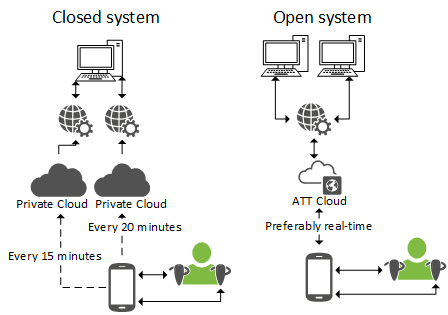
\includegraphics[width=0.9\textwidth]{img/networkloop.png}
    \caption[Image demonstrating a closed cloud system versus an open cloud system]{Image demonstrating a closed system (left) versus an open system (right). A closed system usually has its own (optional) cloud for every device from a different manufacturer, only pushing data but not pulling it. It also (not always) exposes a Web API to allow users to pull the data to their computer. An open system exposes \textit{one} public cloud like the AllThingsTalk cloud with \textit{one} Web API, also allowing 2-way data communication between smartphone and cloud.}
    \label{fig:networkloops}
\end{figure}

\subsection{Research questions}
\label{subsec:researchquestions}
There are a couple of questions that can be asked when combining Bluetooth Low Energy and the Internet of Things, and some of those questions alone could have multiple papers dedicated to them. For example, the matter of security will be a never ending debate, and even more concerns arise when talking about security in the Internet of Things. Another concern is privacy, but since this is very much a gray area, it's hard to formulate a one-sided conclusion on this matter. Some of these concerns will be addressed further in section \ref{sec:concerns}.

The main goals this thesis tries to fulfil are in essence very simple, but of course there are always some other questions that arise when looking at the big picture. These questions can be categorized as following, the questions in bold being the main research questions and the ones in plain text being auxiliary questions:
\begin{itemize}
	\item{\textbf{Can Bluetooth Low Energy wearables be used in an Internet of Things cloud infrastructure?}}
	\item{\textbf{Is is possible to use a smartphone as gateway to communicate with the AllThingsTalk cloud in real-time?}}
	\item{What is Bluetooth Low Energy?}
	\item{What is the difference between Bluetooth Low Energy and Bluetooth Classic?}
	\item{What are the pros and cons of this technology?}
	\item{What types of devices exist in Bluetooth Low Energy and how do they expose their data?}
\end{itemize}

\section{AllThingsTalk}
\label{sec:allthingstalk}
As you've probably already noticed, the company AllThingsTalk has been referenced a couple of times in the previous section. The reason for this is that this thesis is affiliated with the company and is being written for them. The company helped shape the vision of the thesis and offered some very interesting insights and ideas for subjects to write about, subjects which were very interesting for their own use.

AllThingsTalk was founded in July 2013 and their main objective is to `Make IoT ideas happen'. The company is already counting thirteen employees in two different countries, the headquarters being located in Ghent, Belgium. The office in Belgium counts seven people and is heavily focused on research \& development engineering, project management and sales \& marketing. The branch office is located in Belgrade, Serbia with the other six people, and their main focus is platform software development.

\subsection{History}
\label{subsec:atthistory}
AllThingsTalk has come a long way since the start of the company. They've received multiple Research \& Innovation grants from the government, the first being in September 2013 for building an open IoT platform: the AllThingsTalk Cloud. The second grant was received in May 2014, where the goal was to implement pattern recognition in their platform in order to help elderly people stay in their homes for a longer time. A third grant was acquired in February 2015, which was responsible for adding machine learning components to the platform.

Furthermore, they've hit some other major milestones throughout the years. In November 2014 they launched the first set of Rapid Development Kits for Internet of Things, where they added the Intel Rapid Development Kit in April 2015 and the LoRa Rapid Development Kit in November 2015. Other milestones include Internet of Things hackathons, the launch of IOTOPIA.be - a platform to introduce children in secondary schools to Internet of Things - and a LoRa partnership with Proximus, one of the largest telecommunications companies in Belgium.

%\subsection{Products and services}
%\label{subsec:attproductsservices}
%The three main products and services AllThingsTalk offer are guidance, tools and cloud. 
%
%For guidance, they offer IoT innovation workshops and private hackathons. This means that AllThingstalk organizes workshops for companies tailored to their needs, as well as hackathons which involve ideation, prototyping and more.
%
%The second product is tools. AllThingsTalk offers a range of development kits that companies can purchase to accelerate their Internet of Things research. This includes kits like LoRa, Arduino Raspberry Pi, Intel Edison and Windows 10 IoT. `Hackathon in a Box' is also available, which helps companies to organize their own Internet of Things hackathon on their own.
%
%Last but not least is the AllThingsTalk cloud, an Internet of Things prototyping platform which enables companies to connect their devices rapidly to the cloud, instead of hosting their own complicated infrastructure. Not only can this be used to prototype, but the platform is already being used in some very exciting projects like helping the elderly live in their home longer and an ongoing project which provides predictive maintenance in industries with machinery.

% TODO: Wees zo concreet mogelijk bij het formuleren van je
% onderzoeksvra(a)g(en). Een onderzoeksvraag is trouwens iets waar nog
% niemand op dit moment een antwoord heeft (voor zover je kan nagaan).

\chapter{Methodology}
\label{ch:methodology}
\epigraph{``Research is formalized curiosity. It is poking and prying with a purpose.''}{Zora Neale Hurston}
This chapter aims to explain what approaches and methods were used in the making of this thesis. It explains what methods were used for the two major parts of this thesis, being the research \& literature study and the Proof of Concept.

\section{Research and literature study}
\label{sec:researchlit}
Before starting the research, the most important question was `what does AllThingsTalk already know?'. Of course, being a company revolving around Internet of Things, it wouldn't be much use to dedicate a large section of this paper to it. However, some research had to be done about Internet of Things in order to understand some core concepts and technologies that are  used like transfer protocols such as MQTT and AMQP. A more abstract understanding was also needed, being how the Internet of Things works, what it's used for, why it's important and some more. This information is of course easily found online and wasn't of much use to include in this thesis.

That being said, the core subject of the research and literature study is about Bluetooth Low Energy. The research about this technology was done like you would research any other subject. Initially, the plan was to rely heavily on the official documentation of Bluetooth, but since the complete Bluetooth specification is over 2000 pages in length, a more practical approach was to purchase books that explain Bluetooth Low Energy, two of them being REFERENTIE BOEK 1 and REFERENTIE BOEK 2.

There are also training videos to be found on the Bluetooth website as well as various other short introductions to the technology all over the web, which provide a basic and quick understanding about the technology.

\section{Proof of Concept}
\label{sec:poc}
You don't get to know something without actually trying it out, which was one of the biggest focuses of the Proof of Concept. The actual goal of the Proof of Concept was more to provide the Bluetooth Low Energy layer than to connect to the Internet, as AllThingsTalk provides easy-to-use libraries in various language to connect to their platform.

In order to help speed up the learning process and quickly allow me to prototype and try out the technology, various devices were provided which offer a range of Bluetooth Low Energy profiles, services and characteristics, these terms are explained further in chapter \ref{ch:gatt}. These devices will shortly be introduced in chapter \ref{ch:android}.

The first goal of the Proof of Concept was to connect to a Bluetooth Low Energy device and read data on a smartphone. Various examples and repositories with source code provided some interesting insights as to how this API worked. Bluetooth also offers some starter kits to kickstart any project that wants to use Bluetooth Low Energy, including a very comprehensive and easy to use wrapper around the Android Bluetooth API.

Further goals of course include writing data and coupling the Bluetooth layer to the network layer, automatic service discovery and mapping, automatic generation of assets on the online platform and more. The most important concepts on how to do this are elaborated in chapter \ref{ch:android} and the accomplishments are listed in the conclusion, section \ref{sec:conclusion}.


% TODO: Hoe ben je te werk gegaan? Verdeel je onderzoek in grote fasen, en
% licht in elke fase toe welke stappen je gevolgd hebt. Verantwoord waarom je
% op deze manier te werk gegaan bent. Je moet kunnen aantonen dat je de best
% mogelijke manier toegepast hebt om een antwoord te vinden op de
% onderzoeksvraag.


%% TODO: de structuur en titel van deze hoofdstukken hangen af van je 
% eigen onderzoek. Elke fase in je onderzoek kan een eigen hoofdstuk krijgen. Kies telkens een gepaste titel. ``Corpus'' is *GEEN* gepaste titel
\chapter{Bluetooth Low Energy}
\label{ch:ble}
\epigraph{``Bluetooth Low Energy is going to change the way the world connects.''}{Robin Heydon}
Bluetooth has been around for a long time, and with the release of technologies like NFC it seemed like Bluetooth wasn't going to last for much longer. However, Bluetooth Low Energy has breathed new life into Bluetooth and it's now more popular than ever. Originally known as Wibree by Nokia, it was later merged into the Bluetooth standard after much consideration. This technology was built from the ground up to be as energy efficient as possible and will power the Internet of Things for years to come. Exciting updates are also on the way like mesh networking, allowing different nodes in a network to relay data to one another. In this chapter we'll be looking at what Bluetooth Low Energy actually is, what the key differences are between Bluetooth BR/EDR and Bluetooth Low Energy. Also worth investigating are the limitations of Bluetooth Low Energy and how this technology achieves low energy like no other.

\newpage{}

\section{What is Bluetooth Low Energy}
\label{sec:whatis}
In essence, Bluetooth Low Energy is the first open standard that consumes extremely low power. It has been built from scratch and has more things not in common than it does with Bluetooth, so the name can be a little bit confusing. Every component in this specification has been designed to consume as little power as possible, that's why this technology can also be called a `Coin cell' technology. This because a Bluetooth Low Energy enabled device can (theoretically, with normal usage) achieve battery life of around eight months on a coin cell battery. A great example of this are beacons, which can achieve a very long battery life if configured correctly. If fitted with a bigger battery, it can last for over two years. More information about the battery usage and how this low energy is achieved can be found in section \ref{sec:lowenergy}.

However, you might be thinking: if Bluetooth Low Energy is so great, why isn't it replacing other wireless technologies? The main reason for this is because it's very slow and has very little range. A couple of other limitations are present, but these will be more closely looked at in subsecion \ref{subsec:limitations}. Bluetooth Low Energy's main use is intended for Personal Area Networks, with a gateway in range that can relay data to a cloud service in order to connect various devices to the internet.

\section{Key differences between classic Bluetooth}
\label{sec:differencesclassic}
As the diligent reader probably already noticed, it seems that Bluetooth and Bluetooth Low Energy are worlds apart from one another. This is in fact very correct so it's hard to just list some differences and be done with it. In the next two subsections we'll look at why Bluetooth Low Energy is completely different from Bluetooth and should be seen as a new technology in its whole instead of an enhancement to the existing Bluetooth. The key limitations of the Bluetooth Low Energy specification are also addressed further in subsection \ref{subsec:limitations}.

\subsection{A new technology emerges}
\label{subsec:newtechnology}
A lot of authors are looking to compare Bluetooth with Bluetooth Low Energy, but this is an unfair comparison since the use cases for both of these technologies are completely different. As the name suggests, Bluetooth Low Energy is marketed for low energy devices like wearables and sensors, so it isn't here to replace other wireless technologies in the slightest where a continuous flow of data is required. They've also both been built around completely different core principles and have been designed to fulfil these requirements as best as possible.

\subsection{Limitations of Bluetooth Low Energy}
\label{subsec:limitations}
Bluetooth Low Energy doesn't bring all good news, but there are also a few key limitations to the technology, as with everything in life. Because the technology uses very little power, it's fairly easy to understand that the transmit power and transfer speeds aren't anywhere near other wireless technologies. In theory, Bluetooth Low Energy can achieve ranges of up to 65 meters and upcoming updates to the specification prove that this range will be increased even more. However, most manufacturers won't want their peripheral to transmit at such high range, because this will cause increased battery usage in turn. In practice, this range is of course much lower, as walls and even humans wreak havoc on the transmission of data.

Another limitation is the transfer speed. Again, in theory, Bluetooth Low Energy can have a (full packet) transfer speed of up to 1 Mbps\footnote{1 Mbps equals to 100 kilobytes per second.}. If you take into account the actual data contained in said packet and add up all of the overhead that goes into transferring a packet, 5 to 10 KB per second is a much more realistic representation. Knowing this, it's safe to assume that Bluetooth Low Energy won't be replacing WiFi any time soon.

A more concerning limitation is that Bluetooth Low Energy operates in the 2.4 GHz ISM frequency band, the same band that WiFi uses. They've chosen this band because the 2.4 GHz ISM band doesn't require any licensing cost, contributing to the very low chip cost of Bluetooth Low Energy devices. Luckily, Bluetooth Low Energy features an excellent algorithm to avoid major interference from WiFi, as it will avoid any channel that is being heavily used by other technologies.

\section{Bluetooth configurations}
\label{sec:bleconfigurations}
Bluetooth Low Energy is known by a variety of names on the market and while some of them are used to describe the same technology, in a few there's some differences to be found. `Bluetooth Low Energy' is mostly used as a catch-all name and can consist of a few different configurations. Some people assume `classic' or Bluetooth BR/EDR is also Bluetooth Low Energy, but this assumption couldn't be more wrong. If you have a product that specifies that you must have Bluetooth Version 4.0 or later, you're probably dealing with a Bluetooth Low Energy product.

Other names that can commonly be found are Bluetooth Smart (single-mode) and Bluetooth Smart Ready (dual-mode), these are both specifications of Bluetooth Low Energy but have one key difference between each other: backwards compatibility. Bluetooth Smart has been designed to only allow interoperability between itself and Bluetooth Smart Ready products. You'll usually see this configuration in wearable devices that connect to a smart phone, in this case the wearable is a Bluetooth Smart product and the smartphone is a Bluetooth Smart Ready product. Bluetooth Smart Ready on the other hand has been designed to allow communication with Bluetooth, Bluetooth Smart Ready and Bluetooth Smart products. Bluetooth Smart Ready is commonly present in the most recent smartphones, which will allow communication with Bluetooth products like headphones but also Bluetooth Smart products like a smart band. A more comprehensible and orderly overview of these technologies can be found in table \ref{table:configurations}.

\begin{table}[]
\centering
\caption{Compatibility table of Bluetooth specifications}
\label{table:configurations}
\begin{tabular}{|l|l|l|}
\hline
\textit{\textbf{Bluetooth specification}} & \textit{\textbf{Supports BR/EDR}} & \textit{\textbf{Supports BLE}} \\ \hline
\textbf{Pre-v4.0}                   & v                                 & x                              \\ \hline
\textbf{4.x Bluetooth Smart}        & x                                 & v                              \\ \hline
\textbf{4.x Bluetooth Smart Ready}  & v                                 & v                              \\ \hline
\end{tabular}
\end{table}

\section{How low energy is achieved}
\label{sec:lowenergy}
There are a couple of techniques Bluetooth Low Energy uses to achieve low energy consumption. The fact alone that it can run off a 3 volt CR2032 coin cell battery and still retain 8 months of battery life proves that it is indeed a \textit{true} low energy technology. There are a couple of decisions that made it possible to achieve this low amount of energy consumption, some being the following:

\begin{itemize}
\item{\textbf{Use the radio as little as possible.} Keeping the radio on any wireless technology active requires quite a bit of power, which is also the case with Bluetooth Low Energy. By using the radio as little as possible, Bluetooth Low Energy can significantly increase its battery life. At a set interval, devices will broadcast advertising packets on the three advertising channels, which are explained more in section \ref{sec:channels}. After it advertises, it must listen briefly to any connection requests that follow it, in between these events the radio is simply turned off. The radio and the protocol stack, explained more in depth in chapter \ref{ch:protocolstack}, have also been designed to be as fast as possible. An advertising event, connection event, reading a single value of data and acknowledging the event can take as little as 3 milliseconds, which is vital in not only keeping the energy consumption to a minimum, but it also helps passively cool the radio.}

\item{\textbf{Keep packets very small.} Restricting the packet length to a maximum of 47 bytes allows very rapid packet transfers, which in turn contributes to keeping the radio off as much as possible. A maximum size packet of 47 bytes can be transferred in as little as 0.3 milliseconds. Keeping packets small also lowers the complexity of the transmitter and receiver, resulting in much lower power consumption than technologies that allow large packets.}
\end{itemize}

\chapter{The Bluetooth Low Energy protocol stack}
\label{ch:protocolstack}
\epigraph{``I NEED TO LOOK UP A QUOTE FOR THIS CHAPTER''}{Jan Van Braeckel}
Before diving more into the specifics about communication in Bluetooth Low Energy with data packets and advertising packets it's important to know at least some of the fundamentals of the protocol stack that enables devices to communicate with one another. The protocol stack consists of three main parts: the controller, the host and the application. In this chapter we'll be looking at each of the layers, interfaces, protocols and profiles that make up these three parts, giving some insights as to how Bluetooth Low Energy works on a lower level and how data is delegated from layer to layer to build comprehensible communication. Two of the profiles discussed in this chapter however are a fundamental part of Bluetooth Low Energy and thus have their own chapters dedicated to them in order to go into them deeper.

\newpage{}

\section{Controller}
\label{sec:stackController}
At the lowest level in the Bluetooth Low Energy stack, closest to the actual antenna which broadcasts packets, is the controller. The controller manages everything from sending actual data through the radio and the state of the radio. In the following subsection we'll look at the physical layer, which contains circuitry as well as the link layer which sends commands to the physical layer in order to make the process easier through a shared interface.

\subsection{Physical Layer}
\label{subsec:controllerPHY}
The physical layer is the layer responsible for actually sending data over the air. As explained in section \ref{sec:channels}, the physical layer uses the 2.4 GHz ISM band to send and receive its data. In order to avoid interference from WiFi or other technologies that use this band, Bluetooth Low Energy uses frequency hopping with the following algorithm:

\begin{equation*}
\text{newChannel = (currentChannel + hopAmount) mod 37}
\end{equation*}

The hop amount is communicated with both master and slave once a connection has been established, so this hop amount can be different for every connection made and it shouldn't be assumed that this is a fixed number.

\subsection{Link Layer}
\label{subsec:controllerLL}
The link layer is the layer that manages the physical layer. It sends the data the physical layer should send and it also keeps the state of the physical layer, the state machine diagram is shown in figure \ref{fig:llstatemachine}. 

This state machine diagram shows which states the Physical Layer can be in. The Physical Layer can only be in one state at a time, and the diagram shows which states each state can flow into when it's time.

First up is the Standby state, where the Physical Layer doesn't send nor receive any packets. As seen on the diagram, the Standby state can be entered from any other state and can transition into any state except the Connection state.

In the Advertising state, the Physical Layer will only advertise its presence and potential sensor data if configured correctly, this is also known as an advertiser. It also listens to scan requests and can respond to these requests if it wishes to do so. This state can only be entered from the Standby state.

Next up is the Scanning state, where the Physical Layer only listens to advertising packets from other Bluetooth Low Energy devices, this is also known as a Scanner. The Scanning state can only be entered from the Standby state.

Further up is the Initiating state, where the Physical Layer listens to advertising packets from certain devices which have indicated they want to connect to the device, this is also known as an Initiator. The Initiating state can only be entered from the Standby state after the right conditions have been met.

Last but not least is the Connection state. You can see that this state can be entered from both the Advertising and Initiating state. When it is entered from the Advertising state, the device will take on the role of slave or peripheral. When entered from the Initiating state, the device will be seen as the master.

\begin{figure}[h]
    \centering
    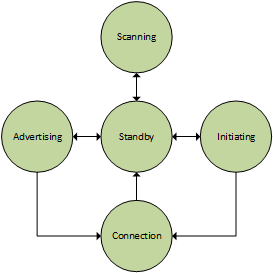
\includegraphics[width=0.5\textwidth]{img/llstate.png}
    \caption{State diagram for the Link Layer state machine}
    \label{fig:llstatemachine}
\end{figure}

\subsection{Host Controller Interface}
\label{subsec:controllerHCI}

\section{Host}
\label{sec:stackHost}

\subsection{Host Controller Interface}
\label{subsec:hostHCI}

\subsection{Logical Link Control and Adaption Protocol}
\label{subsec:hostATTL2CAP}

\subsection{Attribute Protocol}
\label{subsec:hostATT}

\subsection{Security Manager Protocol}
\label{subsec:hostSMP}

\subsection{Generic Access Profile}
\label{subsec:hostGAP}

\subsection{Generic Attribute Profile}
\label{subsec:hostGATT}

\section{Application}
\label{sec:stackApplication}
At the highest level of the protocol stack is the application. As you'd expect, the application is the actual program that embedded software developers will make. It contains logic, calculations and/or the user interface. This application can be coded in a variety of languages and dialects, but most developers will be familiar with C or C++, which is used for a lot of low level applications. An example of such application will be given in chapter \ref{ch:android} for an Arduino 101/Genuino 101 with an Intel Curie chip, which enables Bluetooth Low Energy communication. This Genuino 101 is programmed using the Arduino language which is basically a set of C and C++ functions, so these languages could be used as well to build an application.

\chapter{Generic Access Profile}
\label{ch:gap}
\epigraph{``I NEED TO LOOK UP A QUOTE FOR THIS CHAPTER''}{Jan Van Braeckel}
One of the most important parts in Bluetooth Low Energy, if not most important one, is the Generic Access Profile. This profile determines everything from advertising device presence to continuing to a connection. It specifies rules how devices can and must behave in order to interact with one another and imposes some general rules both devices have to follow. It also supports some modes and procedures to secure the data link, like authentication, bonding, authorization and encryption. In this chapter, we'll look at some general information about the Generic Access Profile like device roles and data channels before taking a look at how advertising, scanning, broadcasting and connections work.

\newpage{}

\section{Roles}
\label{sec:roles}
Every Bluetooth Low Energy device has a one or more roles it can fulfil. Each of these roles have been optimized to perform their task as best it can. First of all there's the Broadcaster role, which only requires a device to have a transmitter and advertising profile. Broadcasters aren't necessarily devices that you can connect to, so manufacturing broadcast only devices could cut down on cost even more as there's no need to have a receiver on these devices. An example of this is a thermostat which constantly broadcasts its temperature.

Secondly there's the Observers, these devices are opposite to broadcasters as they don't require a transmitter. Observers just listen to advertising events and process the data further, without ever making a connection. These devices make perfect gateways for Observers, as a connection will never occur between these two, and the observer can just relay the data to an other collection point.

The last two types of roles are Peripherals and Centrals. These two are the most complex roles as both devices are required to have both a transmitter and receiver. The big difference however is that a Peripheral will always act as a slave in a connection and a Central will always act as a master. This also means that the peripheral will (most of the time) be the least powerful device with the lowest battery life, like a watch or a sensor. It's vital that Peripheral devices don't do the heavy lifting in connections because this would drain the battery too quickly. The Central in a connection is usually a much more powerful device with a better battery life, like a smartphone, tablet or even computers.

\section{Data channels}
\label{sec:channels}
Bluetooth Low Energy uses a number of channels in the 2.4 GHz ISM frequency band. Some of these channels are used for advertising and most of them are used for transferring data once a connection has been made. In total 40 channels are used, 3 of which are used for advertising and the remaining 37 are used for connections. The frequency range starts at 2402 and ends at 2483.5, giving each frequency a range of about 2 MHz to operate on. These channels have been carefully picked to have the least interference possible from WiFi on the advertising channels. Since every connection starts with advertisements it's vital that these packets flow without interference. A visualization of these channels can be found in figure \ref{fig:channelmap}.

In order to make sure that connection packets flow as frequently as possible without having too many dropped packets, Bluetooth Low Energy uses adaptive frequency hopping. This means that at a set interval that the master and slave negotiate with each other, they will switch frequency with a known algorithm, ensuring they'll always end up in the same frequency band. If data doesn't make it through on a given channel, the frequency hop will occur prematurely and both master and slave will move on to the next frequency and resend the packet(s) that weren't acknowledged.

\begin{figure}[h]
    \centering
    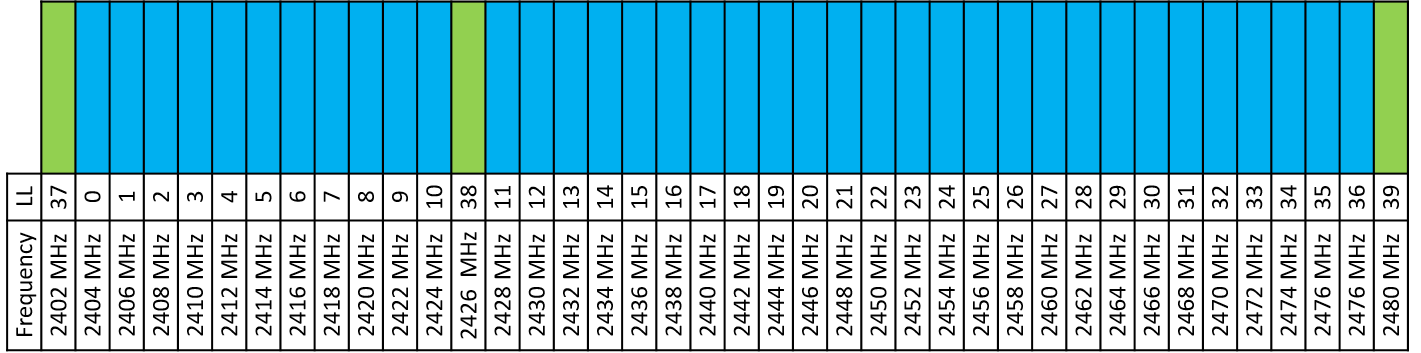
\includegraphics[width=0.9\textwidth]{img/channelmap.png}
    \caption[Image visualizing the Bluetooth Low Energy channel spectrum]{Image visualizing the Bluetooth Low Energy channel spectrum. The green channels are advertising channels while the remaining 37 are used for connections. LL stands for the corresponding number that the link layer assigns to these channels.}
    \label{fig:channelmap}
\end{figure}

\section{Advertising}
\label{sec:advertising}
As quoted a few times before, advertising is one of the most important procedures in Bluetooth Low Energy. A device can be built solely around advertising data, but no device can work without it. Its main purpose is to broadcast the device is present and active so devices can connect with it if the device is connectable, but it can be used for more than that. A typical device will constantly be advertising its state to other devices. This state can be device name, device address and even an (incomplete) list of available services on the device. The advertising interval differs from device to device, but it's easy to conclude that a device with a faster advertising interval will drain battery more quickly than one with a slow advertising interval.

If the device can't fit enough data into the advertising packet, there is a second option to send more data without requiring a connection. Once a device receives an advertising packet, it can send out a Scan Request, acknowledging that it received the previous advertising packet and is listening for extra packets if there are any. The peripheral can then proceed to send a Scan Response with extra data. \colorbox[rgb]{0.2,0.8,0.2}{It's important to note however that a peripheral that uses Scan Requests isn't connectable,} \colorbox[rgb]{0.2,0.8,0.2}{which means that it's perfect for a beacon or any sort of other advertising device.} SOURCE

\subsection{Data format}
\label{subsec:advdataformat}
As discussed in subsection \ref{subsec:controllerLL}, each packet, be it advertising or data, has the same maximum length and structure but the data part of the packet is filled depending on the type of packet that is sent. The data in an advertising packet is filled with AD Types which take up one byte, and the data for that AD Type which is of variable length. An incomplete list of these AD Types together with their definition is found below. A full list of AD Types together with their descriptions can be found on the Bluetooth website\footnote{https://www.bluetooth.com/specifications/assigned-numbers/generic-access-profile} and Bluetooth Core Specification.

\begin{itemize}
	\item {List of Service Class UUIDs (0x02 - 0x07): Helps with finding out the purpose of a device, can contain a complete or partial list of available services on the device.}
	\item {Shortened or Complete Local Name (0x08 \& 0x09): Usually gives a friendly name to a device in UTF-8 format.}
	\item {Service Data (0x16): Represents a GATT service and the data associated with it, this is in essence how a broadcasting only device transfers data.}
	\item {Appearance (0x19): Contains a number representing the external appearance. This can be anything from ``Generic Keyring'' to ``Joystick''.}
	\item {Indoor Positioning (0x25): Helps with mapping BLE devices in a building, can contain coordinates, altitude, floor number and location name.}
	\item {Advertising Interval (0x1A): How often the device advertises its presence.}
\end{itemize}

\section{Broadcasting}
\label{sec:broadcasting}
As discussed in the Advertising section \ref{sec:advertising}, it's possible to have a device that only advertises data and isn't connectable, or its main purpose doesn't rely on connections. This is known as a broadcast device and can be used in broadcasting network topologies. Take for example a radio station, it simply broadcasts its data and it doesn't really matter how many people are listening. When broadcasting, you don't care how many devices can be listening to your data and you shouldn't care about security when advertising data. A great example of this are beacons, which broadcast a very simple payload telling they're there. Infinite amount of devices can listen in on this data communication and use it for their own. Once you need to send sensitive data or only want two-way communication, a connection must be established which uses the GATT Profile to exchange data between master and slave. More information on GATT can be found in chapter \ref{ch:gatt}.

\section{Connections}
\label{sec:connections}
Once a central is ready to connect to a peripheral, it sends a connection request to the peripheral. The peripheral can then accept or deny the request and once accepted, the connection sequence can begin. During the establishment of a connection, a few key rules are established that will stay in place for the remainder of that connection or until both devices agree to change the connection parameters. These rules can be hop frequency, hop amount, what to do when the connection fails and more. Some of these parameters can be changed during the connection lifetime, an example of this is given in section \ref{sec:channels}, where the devices can agree to avoid a given channel for a certain time because there's too much interference. Once a connection has been established, the peripheral will stop advertising its presence since it can only be connected to one central. For the remainder of that connection, both master and slave will exchange data solely with GATT until the connection terminates. The peripheral will then continue once again to advertise its presence.

\chapter{Generic Attribute Profile}
\label{ch:gatt}
\epigraph{``You can have data without information, but you cannot have information without data.''}{Daniel Keys Moran}
At the core of Bluetooth Low Energy communication, the Generic Attribute Profile or GATT is something a client will use in every data request or data push once a dedicated connection has been set up. It defines the way data is transferred in Bluetooth Low Energy and it uses the Attribute protocol, which is the protocol that stores Services, Characteristics, Descriptors and their respective values. In this chapter the general Attribute Profile and Protocol will be discussed, as well as the different data structures that come in to play. An example of an Attribute server will also be given using a standard SIG-approved Profile, as well as why and how one would implement their own Profile, either because the SIG-approved Profiles don't fit the use case or because the manufacturer wants to make the used technology more private.

\newpage{}

\section{Profiles}
\label{sec:profiles}
Profiles in Bluetooth Low Energy are an abstract representation of how a device can be implemented to fill a specific use case. These profiles are purely an example of how things can be done and these can be extended as you want or you can start from scratch and define your own profile. The Heart Rate profile for example defines that the device uses a minimum of two services: the Heart Rate Service and the optional Device Information Service. Its role is a Heart Rate Sensor and it serves as a collector, collecting data and then broadcasting it or sending it to a connected master device.

\section{Services}
\label{sec:services}
All data in Bluetooth Low Energy is accessed through services. You can compare it to simple Object Oriented principles: a service has multiple characteristics and a characteristic belongs to one single service. An example of this is the Bluetooth SIG defined Heart Rate Service. This document defines the way the Heart Rate Service is used and what characteristics are contained in the service. For example, the Heart Rate Service defines 3 characteristics: Heart Rate Measurement, Body Sensor Location and Heart Rate Control Point, only the Heart Rate Measurement is mandatory to include.

A device can host any number of services which are independent of one another. Every service also has its own security options which you can customize. You can set options like encryption for individual services or the device as a whole.

Apart from multiple primary services, a service can also be contained in a parent service, this is then known as a secondary service. However, the secondary service system isn't encountered that often, but it can be useful at times. Take for example a device which has two temperature sensors, one for the outside temperature and one for the battery temperature. The manufacturer could then choose to include the temperature service for the battery as a secondary service of the battery service, this avoids ambiguity.

Apart from the SIG-defined services, a custom service can be designed if the defined services don't meet the expectations of the use case. It's up to the manufacturer to provide documentation for these services or not.

\section{Characteristics}
\label{sec:characteristics}
The actual data of services is contained in characteristics. Every characteristic belongs to a specific service and has a value attached to it. However, it's not because you can see the characteristic, that you don't need special rights to read or write it. A characteristic can specify certain rights like read, write, read uncommitted (where no acknowledgement is sent for the write request) and more. This is something that can be ignored, but an error message will be returned anyway if you try to read a characteristic that isn't readable. These permissions can be used to notify the user interface that it shouldn't allow the user to interact with certain characteristics.

If we take our trusty Heart Rate for example, the Heart Rate Measurement, we can look at the data structure and how the value should be parsed. This characteristic also has some ``Flags'' bits which indicate things like the data type of the value (UINT8 or UINT16) and if certain fields are present or not. Depending on the Flags, there are a couple of values to be found inside this characteristic: Heart Rate Measurement Value, Energy Expended and RR-Interval.

As with services, custom characteristics can also be defined. A template characteristic can be used or the bit structure can be designed from the ground up to accommodate the specific use case.

\section{Descriptors}
\label{sec:descriptors}
If we go down even further, we come to the descriptors. These can optionally accompany characteristics and describe the value of a given characteristic. The descriptors can house very useful data like a description, a valid range of the data and a couple more. If these descriptors are defined, it can greatly help with building up a user interface by only allowing certain values or showing a description for a custom made characteristic, but one shouldn't rely on these descriptors as they're not filled in more often than not.

\chapter{Why Bluetooth Low Energy and Internet of Things}
\label{ch:BLEIOT}
\epigraph{``I NEED TO LOOK UP A QUOTE FOR THIS CHAPTER''}{Jan Van Braeckel}
The Internet of Things is quickly growing and it's already huge, filled with both long-range sensors using LoRa and Sigfox technologies and short-range sensors using WiFi or directly connected with a gateway connected to internet. Why would it then be beneficial to add another spectrum of devices: Bluetooth Low Energy? The main reason for this is because no other technology fills this spectrum of devices yet. Right now, you can compare wireless IOT technologies against 2 axis: power and range, as seen in figure \ref{fig:powerrange}. Before Bluetooth Low Energy, there wasn't really any major technology to fill the Low Energy, Low Range spectrum. One can say that Zigbee or other technologies could fill this end of the spectrum, but none of these are as widely adopted as Bluetooth Low Energy is today. In this chapter we'll further discuss the use cases Bluetooth Low Energy can fulfil in this Low Power, Low Range spectrum as well as briefly introducing its competitors, before ending with what the future holds for Bluetooth Low Energy.

\begin{figure}[h]
\centering
\begin{tikzpicture}

\begin{axis}[axis equal=true,
		ticks=none, axis y line=center, axis x line=middle, axis on top=true,
    xmin=-4.5, xmax=4.5, ymin=-4.5, ymax=4.5,
		xlabel={Power}, ylabel={Range}
] 

\fill[white] (axis cs:0,0) rectangle (rel axis cs:1,1) node [pos=0.5,text=black] {Cellular};

\fill[white] (current axis.right of origin) rectangle (current axis.below origin) node [pos=0.5,text=black] {WiFi};

\fill[white]
    (axis cs:\pgfkeysvalueof{/pgfplots/xmin},\pgfkeysvalueof{/pgfplots/ymax})
    rectangle (axis cs:0,0) node [pos=0.5,text=black] {LoRa, Sigfox};
	
\fill[white]
    (axis cs:\pgfkeysvalueof{/pgfplots/xmin},\pgfkeysvalueof{/pgfplots/ymin})
    rectangle (axis cs:0,0) node [pos=0.5,text=black] {BLE};

\end{axis} 
\end{tikzpicture} 

\caption{Image showing Bluetooth Low Energy's place in the Range vs Power spectrum.}
\label{fig:powerrange}

\end{figure}

\newpage{}

\section{Uses of Bluetooth Low Energy}
\label{sec:usesble}
When looking at the adopted Bluetooth Low Energy profiles and services, as discussed in sections \ref{sec:profiles} and \ref{sec:services}, it's quite easy to find some general use cases that the technology can be used for. Some important use cases are listed below, but are surely not limited to this list:

\begin{itemize}
	\item{\textbf{Quantified Self, Sport and Fitness}: Cycling Power, Cycling Speed and Cadence, Running Speed and Cadence, Body Composition, Heart Rate, Weight Scale}
	\item{\textbf{Health care}: Blood Pressure, Glucose, Continuous Glucose Monitoring, Health Thermometer, Heart Rate and Weight Scale, Pulse Oximeter}
	\item{\textbf{Location and Proximity}: Find Me, Location and Navigation, Proximity, Indoor Positioning}
\end{itemize}

Of course, once we include non-adopted specifications, the list could go on forever with entries being added every day. For example, there's the ``Flower Power''\footnote{http://www.parrot.com/usa/products/flower-power/} device which measures your plant health by monitoring air temperature, soil temperature, soil moisture, soil electrical conductivity and more. It synchronizes with a smartphone that has the Flower Power application paired to the device and synchronizes the data to an online cloud at set intervals, where the data can then be queried with an API  (closed system as seen in figure \ref{fig:networkloops}). A lot of these services aren't included in the adopted specifications, so extending standard Bluetooth profiles with your own can greatly expand the possibilities of the technology. However, if the manufacturer doesn't release the specifications of their device, interoperability with existing apps or integrating that device in other apps will be made very hard.

However, the Flower Power example isn't exactly the best Bluetooth Low Energy use case in existence. For example, what if there's a gardener who plants some of these devices in his/her customers' yards. If the customer isn't home for two weeks, then there's no cellphone to synchronize the data to and the gardener will have to come over to check if the plants need care either way. Some people in the community also thought this was a problem and made a NodeJS gateway application to run on a Raspberry PI or other computer but the product wasn't originally designed for this and the NodeJS gateway leaves a lot to be desired.

\section{Competitors}
\label{sec:competitors}
As the rules of marketing tell us, there aren't (or there are very little) products that have no significant competitors. While Bluetooth Low Energy is trumping its competitors pretty well, it's still worthwhile to look at the these other technologies and what they do.

\subsection{ZigBee}
\label{subsec:zigbee}
ZigBee has been designed from the ground up with automation in mind, as well as Internet of Things. It's not just focused on home automation, but it's also used for smart energy products, health care, equipment monitoring, remote controls and more. Some major technology manufacturers have adopted this technology and are selling home automation kits for people to set up in their homes, like Xiaomi with its Smart Home kit. Another thing ZigBee does very well is mesh networking. Devices can be connected with one another and exchange data without needing additional gateways to fetch the data. However, the problem with ZigBee is that the platform is completely open and changes can be made for it as the manufacturer wishes. So it might happen that two devices with a ZigBee chip aren't even able to communicate with one another.

\subsection{Z-Wave}
\label{subsec:zwave}
Another wireless technology that is built completely for home automation is Z-Wave. The major difference between ZigBee and Z-Wave however, is that the Z-Wave technology isn't open. This is both good and bad because it's not open at all to development, you simply take the technology as it comes and no flexibility is offered beyond that point. For the consumer this is beneficial however, ensuring interoperability between Z-Wave devices, since Z-Wave also features mesh networking.

\subsection{ANT}
\label{subsec:ant}
ANT is another good example of a Bluetooth Low Energy competitor. This is again a proprietary technology and was built with sensor networks in mind. It features powerful mesh networking as well as star, tree and point-to-point networks, allowing all kind of networks to be used in unison.

\section{Other wireless technologies}
\label{sec:othertechnologies}
There are quite a bit of other technologies that can be used to power the Internet of Things, discussing all of them would take a paper of its own. Some of these technologies and protocols are X10 (home automation), KNX (home automation) and M-bus (industry). Other technologies, not necessarily in the Low Energy/Low Range spectrum are LoRa (Long Range), GPRS (General Packet Radio Service) and Sigfox.

\section{Future of Bluetooth Low Energy}
\label{sec:futureble}
Bluetooth Low Energy has been an exciting technology from the start and is gaining popularity at a very rapid rate. While the Bluetooth 4.0 specification brought Bluetooth Low Energy to life, some very much needed updates have made it to the Bluetooth specification, which is now at version 4.2. Bluetooth 4.1 brought improved consumer usability with better co-existence between Bluetooth Low Energy and Bluetooth BR/EDR, as well as increased data exchange rate and more flexibility for the developers. The 4.1 specification also brought IP-based connections to Bluetooth Low Energy. In essence, a device can directly communicate over internet once it's been connected to a gateway that has internet access, like a smartphone.

The newest update, Bluetooth 4.2, brings yet more changes to the Bluetooth specification. It brings improved speeds yet again, support for IPv6, 6LoWPAN (IPv6 over Low power Wireless Personal Area Networks) and improved security.

The Bluetooth SIG is constantly working on Bluetooth Low Energy, and it has been announced that the range would be significantly improved. They also brought mesh networking to the table, just like ZigBee, Z-Wave and ANT. These improvements will bring even more use cases to Bluetooth Low Energy, the main one being home automation.

\chapter{Building an Android gateway}
\label{ch:android}
\epigraph{``I NEED TO LOOK UP A QUOTE FOR THIS CHAPTER''}{Jan Van Braeckel}
With all of the previous chapters, a good idea and base has been formed as to what Bluetooth Low Energy is and why it would be valuable to integrate it into an Internet of Things environment.

This chapter aims to provide a practical approach to answering some of the research questions stated in bold in subsection \ref{subsec:researchquestions} through a Proof of Concept. The Proof of Concept concerns building an Android application that can successfully connect, communicate and act as a gateway for Bluetooth Low Energy devices. First of all, the devices that were used in the making of this application will be talked about more in detail before looking at how one would implement a gateway for Android. As this is a prototype, a lot of optimizations have to be made and the method used might not be the most ideal one. Methods on one of the ways to implement this on a large scale will be given in section \ref{sec:futurework}.

\newpage{}

\section{Goal}
\label{sec:pocgoal}
The general goal for this Proof of Concept is to build a rough Android application that can connect with multiple Bluetooth Low Energy devices simultaneously, read data and write data. It should also be possible to register the smartphone as a gateway in an Internet of Things cloud, in this case the AllThingsTalk developer cloud. The application has to create devices it connects to on the platform and add its assets, sensors and actuators. Once the data is read on the device, it should also send that data to the correct asset on the online platform. Once this is achieved, the next goal is to enable two-way communication, not only sending data to the platform but also receiving data and sending it to the right device, sensor or actuator.

\section{Used devices}
\label{sec:devices}
Before going in depth on how to implement and use the Bluetooth API for Android and connect the devices to an online platform, it's interesting to go over the devices that were used in the making of this Proof of Concept. In order to quickly prototype and simulate the `real' life at the same time, a mix of consumer and both development devices were used. This was mainly to speed up the development process as certain development devices allow you to easily write your own application as discussed in section \ref{sec:stackApplication}.

\subsection{Nexus 5}
\label{subsec:nexus}
The most important device for developing the gateway is of course a smartphone. It's important that the smartphone used features at least Bluetooth v4.0, as v4.0 and up started to support Bluetooth Low Energy.

By all means, another device than the Nexus 5 could be used to make a gateway. It was just used because it was the best device to my disposal that suited the use case. The Nexus 5 features Bluetooth v4.0, but using a device that has Bluetooth v4.2 won't limit the possibilities in any way since Bluetooth Low Energy is backwards compatible.

\subsection{Arduino 101 / Genuino 101}
\label{subsec:arduino101}
One of the most popular microcontrollers is the Arduino. For this use case, a Genuino 101\footnote{https://www.arduino.cc/en/Main/ArduinoBoard101} (in Europe, Arduino 101 in America) was used because it features an Intel Curie System on Chip. This Intel Curie module, amongst a 6 axis gyroscope and accelerator, features a Bluetooth Low Energy module which makes it ideal for fast prototyping since it's easy to create an application with the Arduino IDE without requiring a lot of set-up.

Besides the board, some additional modules and sensors were used to create an application. For this use case, a very simple application was made based on an existing Heart Rate Monitor application from Arduino\footnote{https://www.arduino.cc/en/Tutorial/Genuino101CurieBLEHeartRateMonitor}.

The adapted application monitors a rotary switch and if connected to a master, it will notify the master every second with the value of the switch. It reports this value through the standard defined Heart Rate service and Heart Rate Measurement characteristic. In a real scenario heart rate wouldn't be measured with a rotary switch, but since this is a prototype it's the easiest solution. To give the device an actuator as well as a sensor, a simple custom service and characteristic were made that just enable or disable a digital device by writing 0 or 1 to the characteristic. The source code of the adapted example can be found in the appendix.

\subsection{Flower Power}
\label{subsec:flowerpower}
In order to have a consumer device to test with, the Flower Power was used. This is a handy little gadget filled with sensors that connects to an application on a smartphone which monitors your plant. It notifies the user when the plant should be watered, if it needs to be moved because it has too little sunlight, if it's too hot or too cold or if its soil isn't fertile enough.

This device features a lot of custom services and characteristics, so it's a very good test device to find out if it's viable to easily support these kind of devices as well. Luckily the Flower Power has good documentation available\footnote{http://developer.parrot.com/docs/flowerpower/FlowerPower-BLE.pdf} so that prevented a lot of reverse engineering and extra time and effort.

\subsection{MetaWear CPRO}
\label{subsec:metawearcpro}
For the last device, a MetaWear CPRO from MbientLab\footnote{https://store.mbientlab.com/product/metawear-cpro/} was used. This is another device destined for prototyping and features a large range of sensors. On top of that, it also runs off a coin cell battery, is very small and even allows developers to write their own firmware or expand the board. It features a temperature sensor, light sensor, a 10 axis motion sensor (gyroscope, magnitude, barometer) and the MetaWear CPRO used for this thesis is also fitted with a buzzer.

\section{Android programming}
\label{sec:androidprogramming}
In this section, the most important parts in building a gateway for Android will be discussed. Everything from building the Bluetooth layer to the network layer will be talked about and it will give a good overview of how all these APIs can work together. The full source code for the application is available on \texttt{GITHUB(LINK)}. This application is a working prototype to bridge Bluetooth Low Energy to the AllThingsTalk developer cloud.

\subsection{Bluetooth layer}
\label{subsec:bluetoothlayer}
As a starting point, the first goal is to get the Bluetooth layer working. In order to get a kick start, the Bluetooth group exposes an Application Accelerator\footnote{https://www.bluetooth.com/develop-with-bluetooth/developer-resources-tools/app-acc-2} that's very easy to use and provides a solid layer above the Android Bluetooth API, making Bluetooth more friendly to use.

However, it's still important to know how the Bluetooth API of Android works and it will save quite a bit of time down the road when debugging a problem.

The starting point for using Bluetooth Low Energy is the \texttt{BluetoothManager} class. After checking Bluetooth compatibility and acquiring the right permissions, this is where all communication will start. The \texttt{BluetoothManager} can be acquired by requesting the \texttt{Context.BLUETOOTH\_SERVICE} system service from the hosting activity which will return an object if it's compatible and permissions have been acquired, or \texttt{null} if it can't return the manager.

\texttt{BluetoothManager} is a high level class used to do overall Bluetooth Management, but it also exposes the \texttt{BluetoothAdapter} class. This class allows for device discovery, querying already bonded Bluetooth devices, initiating a connection using a MAC address and it also allows for scanning Bluetooth Low Energy devices.

Once scanning has been initiated, callbacks will be reported on the \texttt{ScanCallback} interface which exposes a \texttt{ScanResult} object. This object exposes the very important \texttt{BluetoothDevice} member. This device can be queried for the device address, which in turn can be used to initiate a connection. Essentially, connecting to the device means getting a reference to its GATT server - described in chapter \ref{ch:gatt} - which exposes all of the data on the device.

The \texttt{BluetoothGatt} class allows exposes everything that has to do with data. It allows discovering services, its characteristics and its descriptors. It also allows reading data, writing data, enabling or disabling notifications, reading RSSI (signal strength) and more. As with the \texttt{ScanCallback}, the \texttt{BluetoothGatt} class also requires a callback interface to bring data to the application, as all communication in Bluetooth Low Energy happens asynchronously. Once this interface has been implemented, it's simply a task of delegating the data to different parts of the application and displaying it on the screen.

\subsection{Network layer}
\label{subsec:networklayer}
The network layer can differ from architecture to architecture, but the steps used to connect to the AllThingsTalk developer cloud will be discussed here. There are two kinds of clients that can interact with the cloud: a gateway and a device. The difference between these two is that a gateway can register and update multiple devices, but a device can only register and update itself. It makes sense that when using a smartphone, it should be configured as a gateway since it can connect with multiple devices.

First things first, the smartphone has to be registered as a gateway before being able to send any data. The first step is to create the gateway as an orphan on the platform by sending a POST request to \texttt{https://api.smartliving.io/gateway} with a UID (unique identifier, in this case the MAC address of the smartphone), the name of the gateway (in this case the device name, Nexus 5) and the assets, which allow the gateway to be configured from the online portal.

Once this procedure is finished, the smartphone is an orphan in the platform and has to be claimed within 30 seconds before time-out. In order to check if the gateway has been registered, a POST request can be sent to the same URI and once the device has been claimed the response will contain the gateway id. It's a good idea to then save the gateway id on the device so the claim procedure doesn't have to take place every time the application starts. The gateway can then be used to add assets to the online platform. This can be done by sending a PUT request to \texttt{https://api.smartliving.io/device/\_deviceId\_/asset/\_assetId\_/}. The \texttt{deviceId} and \texttt{assetId} are variables that should be carefully chosen so when data is received, the device knows what to do with it. To easily identify where the data should flow, the \texttt{deviceId} is determined by the connected Bluetooth device's unique address. The \texttt{assetId} is a combination of the Bluetooth Service UUID and the Bluetooth Characteristic UUID.

After adding assets, the only thing left is to send actual data. This is done using the MQTT protocol, though HTTP can be used but MQTT is the preferred method. The MQTT protocol is a machine-to-machine protocol optimized for small sensors and mobile devices, which makes it ideal for an Internet of Things infrastructure. It's basically a very simple publisher/subscriber client, where a publisher publishes data to a topic and a subscriber can listen to topics to get updates. So sending and receiving data from the platform can simply be done by sending data to the right topic and subscribing to the topic the client wants to get updates from, in this case all topics are subscribed to in order to receive all asset state updates. In order to make this communication easier, the Paho Java Client library\footnote{https://eclipse.org/paho/clients/java/} was used.

\subsection{User interface}
\label{subsec:userinterface}
This part of the application is the most flexible one and doesn't need a whole lot of explanation since everybody will use a different user interface. The interface used for this prototype looks very simple and is in fact pretty easy to implement. This because most of the work has gone into the network and Bluetooth layer, and the user interface is just something to route the data through.

The first screen is a \texttt{RecyclerView} in a \texttt{SwipeRefreshLayout}. The swipe to refresh layout serves to scan, as it's not that efficient to have the device scanning for connections all the time. It will scan for a set amount of seconds and fill the \texttt{RecyclerView} with any devices it finds, displaying the device name, device address and RSSI (signal strength).

Once a device has been chosen, a new fragment opens with more information about the device. At the top of the screen the device name, device address and RSSI are still displayed. The rest of the screen is filled up using an \texttt{ExpandableListView} which displays all Services in the first level and the Characteristics in the second. The component has been modified so it can expand to three levels, this to accomodate extra information about a Characteristic. Once a Characteristic is expanded, the third level opens which displays the data type, properties (read, write, write no response, ...) and three buttons. The buttons serve to toggle notifications, read and write data. Once data has been read, additional info will be displayed in this third level such as the hexadecimal value, string value, decimal value and timestamp of the last time the data was updated.

\chapter{Discussion}
\label{ch:discussion}

\section{Conclusion}
\label{sec:conclusion}

\section{Concerns}
\label{sec:concerns}

As with every technology, concerns arise once it starts to become popular. Internet of Things and Bluetooth Low Energy are no exception to this and have caused a fair bit of commotion.

First of all is a big problem: security. There are numerous articles being written the last couple of years that would make you wonder if the Internet of Things is even worth it. To give a couple of examples, there is an Internet of Things search engine called Shodan\footnote{https://www.shodan.io/} which allows users to browse unsecured internet-enabled webcams, even baby monitors \citep{porup20162, stanislav2015}. Even the US Intelligence Community has placed Internet of Things on their watch list and believe it is a very big threat \citep{clapper2016}.

Two hackers have done something that might alarm even more people. They have succeeded in hacking an internet-enabled car, gaining control a lot of the car's functions \citep{greenberg2015}. To demonstrate this, the process was documented as a man was driving with an SUV on the highway with the hackers miles away with their laptops. They were able to blast the air conditioning, put pictures on the car display, turn on the radio, spray wind shield wiper fluid and they could even kill the engine of the car. It didn't stop there as they were even able to steer the car while it was in reverse and disable the brakes at low speeds. After this incident, about 1.4 million vehicles were recalled for a software update \citep{kessler2015}. Numerous other cars were also exposed for hackers like the Tesla Model S, certain BMW vehicles, Rolls-Royce vehicles and Mini vehicles \citep{hirsch2015}.

Bluetooth Low Energy doesn't stay under the radar either, as it's increasingly gaining popularity and thus, gaining suspicion. With a cheap phone and a small application, it is possible to locate devices around the smartphone and see what they are. This can be an issue because burglars could simply walk around with this application installed and check which houses have a lot of technology worth stealing \citep{ashford2015}. China has even banned the use of internet-connected wearable technology as it could give the soldiers' position away during combat \citep{bbcnews2015}.

Some students at the University of Illinois have also used the gyroscope and accelerometer of a smartwatch to detect what the user is typing on an ordinary or laptop keyboard \citep{iyer2015, wang2015mole}.

\section{Future work}
\label{sec:futurework}

% TODO: Trek een duidelijke conclusie, in de vorm van een antwoord op de
% onderzoeksvra(a)g(en). Reflecteer kritisch over het resultaat. Zijn er
% zaken die nog niet duidelijk zijn? Heeft het ondezoek geleid tot nieuwe
% vragen die uitnodigen tot verder onderzoek?



\bibliographystyle{apa}
\bibliography{tin-bachproef}

%%---------- Back matter -------------------------------------------------

\listoffigures
\listoftables

\end{document}
